\documentclass[10pt,a4paper]{article}

\usepackage[english]{babel}
\usepackage[utf8]{inputenc}
\usepackage[T1]{fontenc}
\usepackage[a4paper, margin=2cm]{geometry}
\usepackage{amsmath,amsfonts,amssymb}
\usepackage[colorlinks]{hyperref}
\usepackage{multicol}
\usepackage{graphicx}
\usepackage{float}
\usepackage{booktabs}
\usepackage{fancyhdr}
\pagestyle{fancy}
\fancyhead[L]{02460-2026 Mini-project 3}
\fancyhead[R]{s232268, s242875, s253009 \& s257470}
\usepackage{listings}
\usepackage{xcolor}

\definecolor{codegreen}{rgb}{0,0.6,0}
\definecolor{codegray}{rgb}{0.5,0.5,0.5}
\definecolor{codepurple}{rgb}{0.58,0,0.82}
\definecolor{backcolour}{rgb}{0.95,0.95,0.92}

\lstdefinestyle{mystyle}{
    backgroundcolor=\color{backcolour},
    commentstyle=\color{codegreen},
    keywordstyle=\color{magenta},
    numberstyle=\tiny\color{codegray},
    stringstyle=\color{codepurple},
    basicstyle=\ttfamily\footnotesize,
    breakatwhitespace=false,
    breaklines=true,
    captionpos=b,
    keepspaces=true,
    numbers=left,
    numbersep=5pt,
    showspaces=false,
    showstringspaces=false,
    showtabs=false,
    tabsize=2,
    upquote=true
}

\lstset{language=Python, style=mystyle}

\begin{document}

% -----------------------------------------------------------------------
% PAGE 1 — Main text (single page limit)
% -----------------------------------------------------------------------
\section*{Mini-project 3 in Advanced Machine Learning (02460)}
\textbf{Zhenlin Xie (s232268), Ignacio Ripoll Gonz\'alez (s242875), Alexander Hellberg Yanci (s253009), Eugene Ratkovich (s257470)}

\begin{multicols}{2}

\subsection*{Model}
The \textbf{encoder} applies $K{=}3$ message-passing (MP) layers to the node features $\mathbf{x}_v \in \mathbb{R}^7$, producing node embeddings $\mathbf{h}_v \in \mathbb{R}^{64}$ with residual connections. A sum-pooling readout gives a graph embedding $\mathbf{h}_G$, from which two linear heads produce the posterior parameters $\boldsymbol{\mu}, \log\boldsymbol{\sigma}^2 \in \mathbb{R}^{32}$.

The \textbf{decoder} receives a latent sample $\mathbf{z} \sim q(\mathbf{z}|G) = \mathcal{N}(\boldsymbol{\mu}, \text{diag}(\boldsymbol{\sigma}^2))$ concatenated with a normalised node count and passes it through an MLP to produce upper-triangular logits, from which independent Bernoulli edge probabilities are read off. The adjacency is symmetrised and self-loops removed.

The \textbf{training objective} is the ELBO with $\beta$-weighted KL divergence:
\[
\mathcal{L} = \mathbb{E}_{q(\mathbf{z}|G)}\!\bigl[\log p(A|\mathbf{z})\bigr] - \beta\,\mathrm{KL}\!\bigl(q(\mathbf{z}|G)\|p(\mathbf{z})\bigr),
\]
where $p(A|\mathbf{z})$ factorises over edges as independent Bernoulli and $p(\mathbf{z})=\mathcal{N}(\mathbf{0},\mathbf{I})$.
Training used Adam ($\eta{=}10^{-3}$, $\beta{=}1.0$, batch 32) with early stopping (patience 30); the model converged in 79 epochs.

\subsection*{Baseline}
For each generated graph the Erd\H{o}s-R\'enyi baseline (i) samples $N$ from the empirical node-count distribution of the training graphs, (ii) computes the link probability $r$ as the mean density of training graphs with exactly $N$ nodes, and (iii) samples $G(N,r)$.

\subsection*{Evaluation}
Novelty and uniqueness are computed by hashing all graphs with the Weisfeiler-Lehman (WL) algorithm (\texttt{networkx.weisfeiler\_lehman\_graph\_hash}) and resolving collisions with exact isomorphism checks (\texttt{networkx.is\_isomorphic}).

\begin{center}
\small
\begin{tabular}{lccc}
\toprule
 & Novel & Unique & Novel+Unique \\
\midrule
ER baseline     & 100.0\% & 99.7\% & 99.7\% \\
Deep model      & 100.0\% & 100.0\% & 100.0\% \\
\bottomrule
\end{tabular}
\end{center}

Both models are fully novel; the deep model is also perfectly diverse.
Figure~\ref{fig:statistics} compares degree, clustering coefficient, and eigenvector centrality across the training set, ER baseline, and deep model using shared histogram bins.
The deep model's degree distribution is closer to the training data than the ER baseline's,
though pairwise KS tests confirm statistically significant differences in all three statistics for both models vs.\ training.

\end{multicols}

\begin{figure}[H]
    \centering
    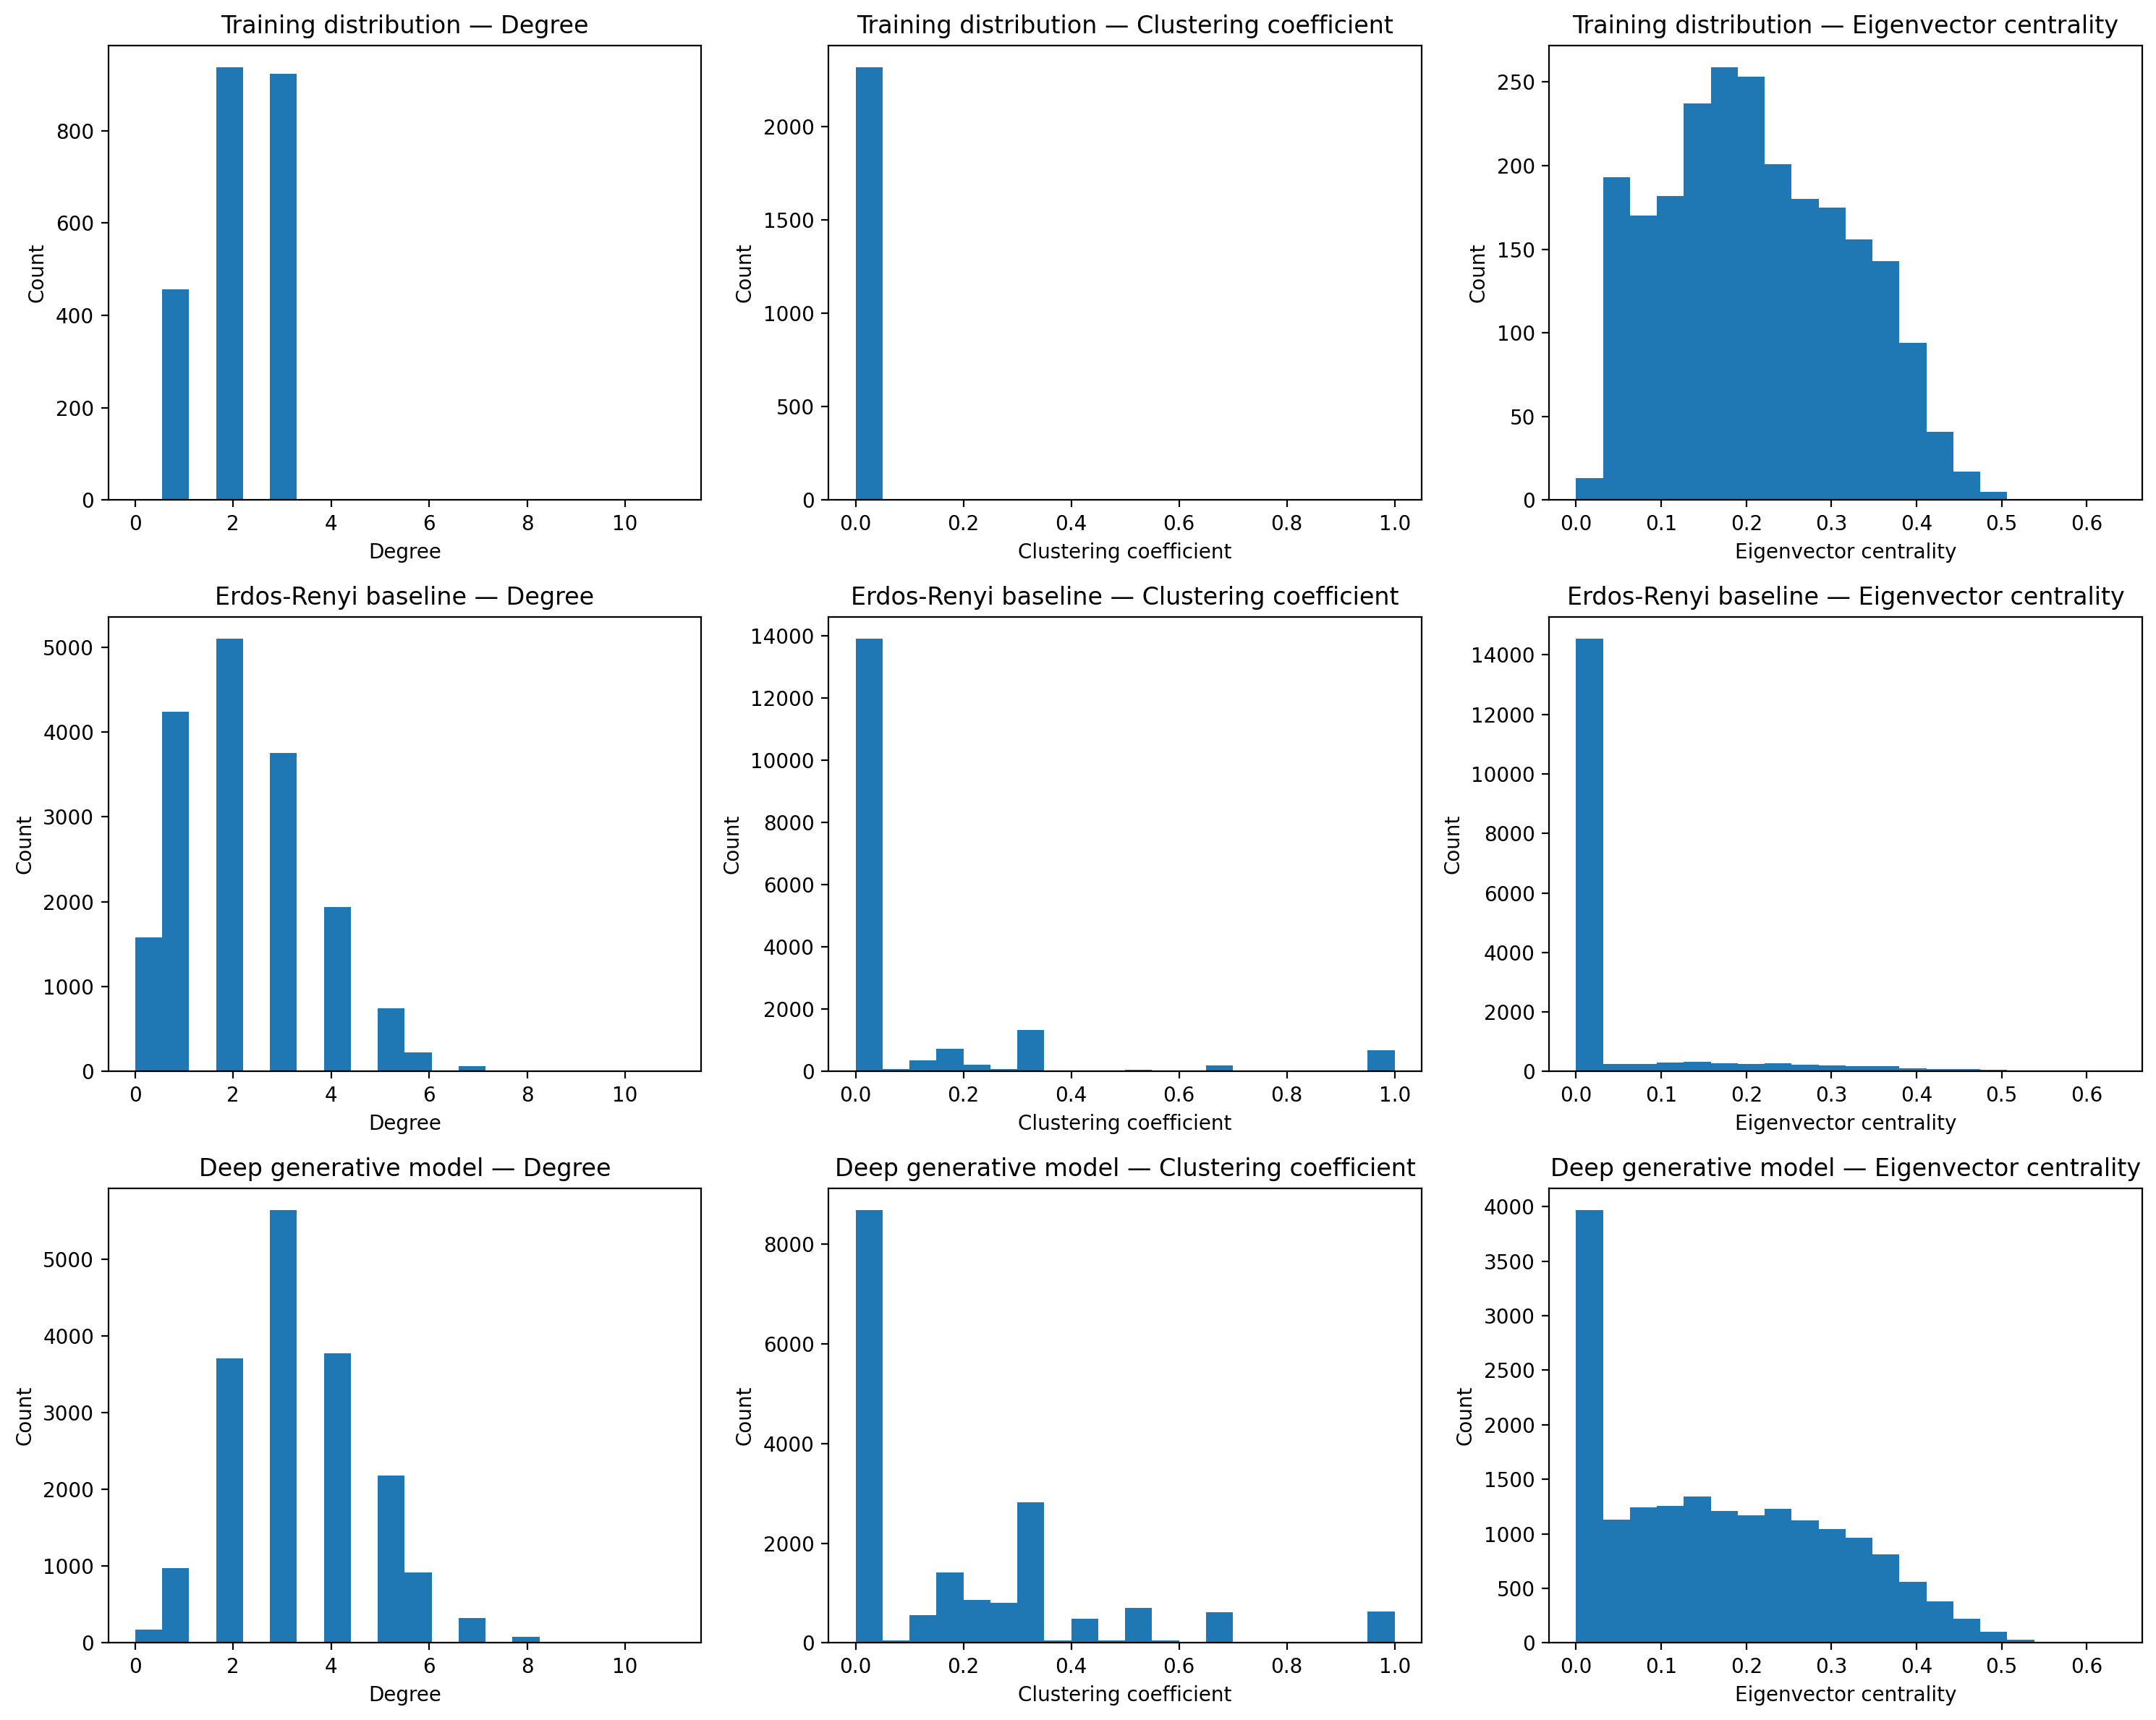
\includegraphics[width=\linewidth]{outputs/figures/graph_statistics_3x3.png}
    \caption{Histogram comparison (shared bins per statistic) of node degree, clustering coefficient, and eigenvector centrality for training data, ER baseline, and deep-model samples.}
    \label{fig:statistics}
\end{figure}

\begin{figure}[H]
    \centering
    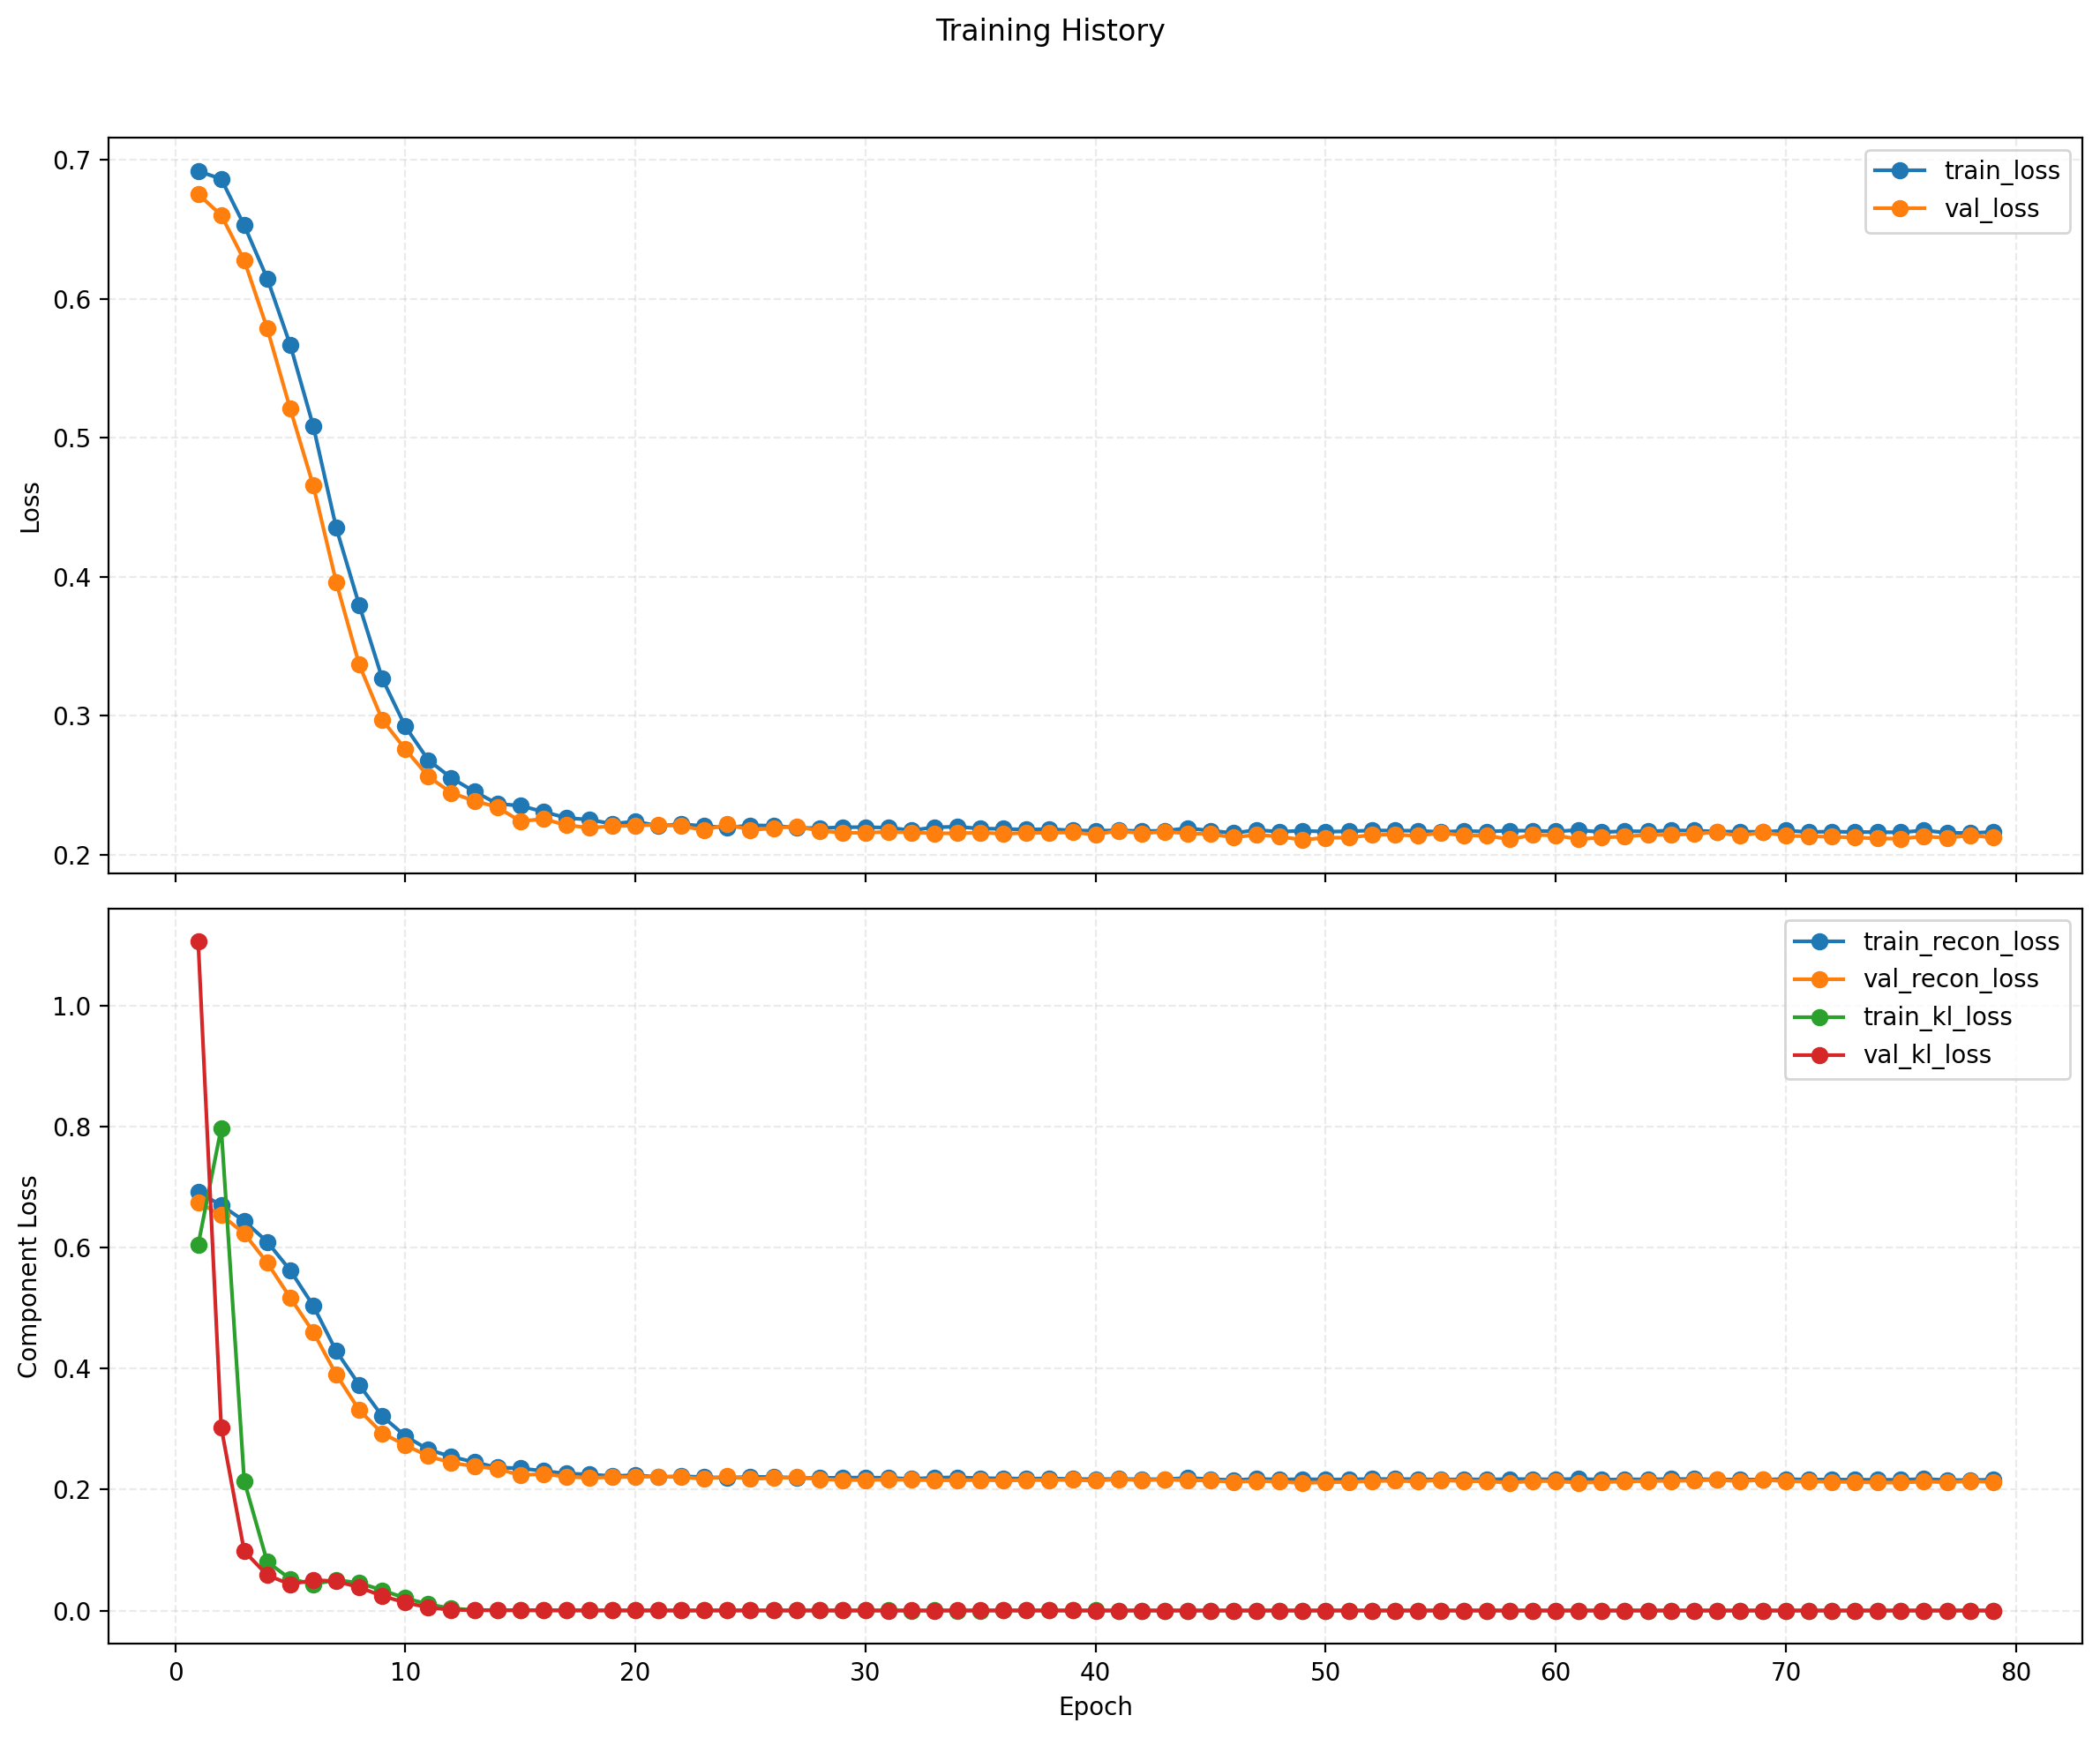
\includegraphics[width=0.72\linewidth]{outputs/figures/training_history.png}
    \caption{Training history: total loss (top) and reconstruction / KL components (bottom) over 79 epochs.}
    \label{fig:training-history}
\end{figure}

% -----------------------------------------------------------------------
% Unlimited pages: references
% -----------------------------------------------------------------------
\newpage
\begin{thebibliography}{9}

\bibitem{kipf2016vgae}
T.~N. Kipf and M.~Welling,
``Variational Graph Auto-Encoders,''
\textit{NIPS Workshop on Bayesian Deep Learning}, 2016.

\bibitem{gilmer2017mpnn}
J.~Gilmer, S.~S. Schütt, G.~E. Hinton, M.~Welling, and D.~Dürr,
``Neural Message Passing for Quantum Chemistry,''
\textit{Proceedings of ICML}, 2017.

\bibitem{debnath1991mutag}
A.~K. Debnath, R.~L. Lopez de Compadre, G.~Debnath, A.~J. Shusterman, and C.~Hansch,
``Structure-activity relationship of mutagenic aromatic and heteroaromatic nitro compounds,''
\textit{Journal of Medicinal Chemistry}, 34(2):786--797, 1991.

\bibitem{morris2020tudataset}
C.~Morris et al.,
``TUDataset: A collection of benchmark datasets for learning with graphs,''
\textit{ICML Workshop on Graph Representation Learning}, 2020.

\bibitem{shervashidze2011wl}
N.~Shervashidze, P.~Schweitzer, E.~J. van Leeuwen, K.~Mehlhorn, and K.~M. Borgwardt,
``Weisfeiler-Lehman Graph Kernels,''
\textit{Journal of Machine Learning Research}, 12:2539--2561, 2011.

\end{thebibliography}

% -----------------------------------------------------------------------
% Single page of well-formatted code snippets
% -----------------------------------------------------------------------
\newpage
\subsection*{Code Snippets}

\begin{lstlisting}[caption={Message-passing encoder with sum-pooling readout (model\_gvae.py).}]
class GraphEncoder(nn.Module):
    def __init__(self, cfg: GraphVAEConfig):
        super().__init__()
        self.input_proj = nn.Linear(cfg.num_node_features, cfg.hidden_dim)
        self.mp_layers = nn.ModuleList([
            GCNConv(cfg.hidden_dim, cfg.hidden_dim)
            for _ in range(cfg.num_message_passing_steps)
        ])
        self.mu_head     = nn.Linear(cfg.hidden_dim, cfg.latent_dim)
        self.logvar_head = nn.Linear(cfg.hidden_dim, cfg.latent_dim)

    def forward(self, x, edge_index, batch):
        h = F.relu(self.input_proj(x))
        for layer in self.mp_layers:
            h = F.relu(layer(h, edge_index)) + h  # residual
        h_G = global_add_pool(h, batch)            # sum-pooling
        return self.mu_head(h_G), self.logvar_head(h_G)
\end{lstlisting}

\begin{lstlisting}[caption={MLP decoder: latent code to upper-triangular adjacency logits (model\_gvae.py).}]
class GraphDecoder(nn.Module):
    def __init__(self, cfg: GraphVAEConfig):
        super().__init__()
        in_dim = cfg.latent_dim + (1 if cfg.use_size_conditioning else 0)
        out_dim = cfg.max_nodes * (cfg.max_nodes - 1) // 2
        self.mlp = nn.Sequential(
            nn.Linear(in_dim, cfg.hidden_dim), nn.ReLU(),
            nn.Linear(cfg.hidden_dim, cfg.hidden_dim), nn.ReLU(),
            nn.Linear(cfg.hidden_dim, out_dim),
        )

    def forward(self, z, num_nodes=None):
        if num_nodes is not None:
            z = torch.cat([z, num_nodes.unsqueeze(-1)], dim=-1)
        return torch.sigmoid(self.mlp(z))   # edge probabilities
\end{lstlisting}

\begin{lstlisting}[caption={ELBO loss with beta-weighted KL (train\_gvae.py).}]
def elbo_loss(recon_probs, target_adj, mu, logvar, beta=1.0):
    # Binary cross-entropy over upper-triangle edges
    recon = F.binary_cross_entropy(recon_probs, target_adj, reduction='mean')
    # KL divergence: -0.5 * sum(1 + logvar - mu^2 - exp(logvar))
    kl = -0.5 * torch.mean(1 + logvar - mu.pow(2) - logvar.exp())
    return recon + beta * kl, recon, kl
\end{lstlisting}

\begin{lstlisting}[caption={WL-hash-accelerated novelty and uniqueness computation (metrics.py).}]
def compute_novelty_metrics(generated_graphs, train_graphs):
    train_buckets = build_hash_buckets(train_graphs)   # WL hash -> [Graph]
    unique_idx    = set(unique_graph_indices(generated_graphs))
    novel_flags   = [is_graph_novel(g, train_buckets) for g in generated_graphs]
    n = len(generated_graphs)
    num_novel  = sum(novel_flags)
    num_unique = len(unique_idx)
    num_nu     = sum(1 for i, nov in enumerate(novel_flags) if nov and i in unique_idx)
    return NoveltyMetrics(n, num_unique, num_novel, num_nu,
                          num_unique/n, num_novel/n, num_nu/n)

def build_hash_buckets(graphs):
    buckets = {}
    for g in graphs:
        h = nx.weisfeiler_lehman_graph_hash(g)   # WL hash
        buckets.setdefault(h, []).append(g)
    return buckets
\end{lstlisting}

\end{document}
